\chapter{Planning and Budget}
\label{ch:planning-and-budget}

\section{Planning}
The planning of this work covers from the moment the proposal for the teaching commission began
to be made until the moment the work is presented publicly. Of course there are some milestones
that are fixed in time such as \textbf{the presentation of the proposal}, \textbf{the presentation of the dissertation}
and \textbf{the defense of the work}. Therefore planning revolves around these milestones \textit{(IDs
3, 4 and 5 from \cref{fig:planning-sheet})}.

\subsection{Presentation of the Proposal}
The acceptance of the proposal includes the first tasks \textit{(IDs
6-8 from \cref{fig:planning-sheet})} in which a small investigation is done on the
topics of interest and it is decided what the objectives to be pursued of the work will be.

In addition, it also includes the formal preparation of the proposal that will be delivered to the
management of the computer engineering school for evaluation.

\subsection{Presentation of the Dissertation}
To consider the presentation of the dissertation as complete, it is necessary to carry out the main
tasks \textit{(IDs 9-34 from \cref{fig:planning-sheet})} of the work, in our case they are to
carry out the corresponding research to understand the scope of the proposed objectives, to propose a
solution and to obtain a few relustados that can be empirically testable. So that we can evaluate our
solutions. And, of course, prepare the corresponding documentation that reflects all the work done.

\subsection{Defense of the Work}
The defense of the project corresponds to those tasks \textit{(IDs 34-36 from \cref{fig:planning-sheet})}
subsequent to the delivery of the dissertation and that have to do with public defense in which the work carried out is evaluated.

\bigskip
So as you can see the main project statistics are shown in \cref{tb:planning-stats}.

\begin{table}
    \caption[Statistics of the main project tasks]{Statistics of the main project tasks.}
    \label{tb:planning-stats}
    \centering
    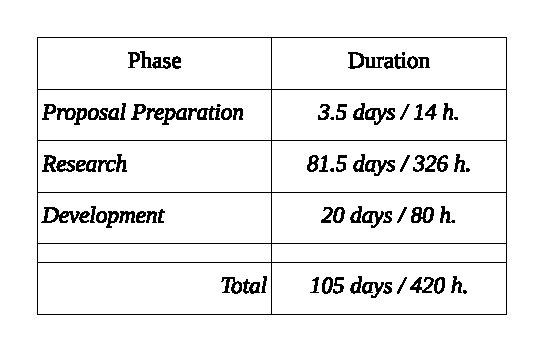
\includegraphics{images/planning-stats.pdf}
\end{table}

\begin{figure}
    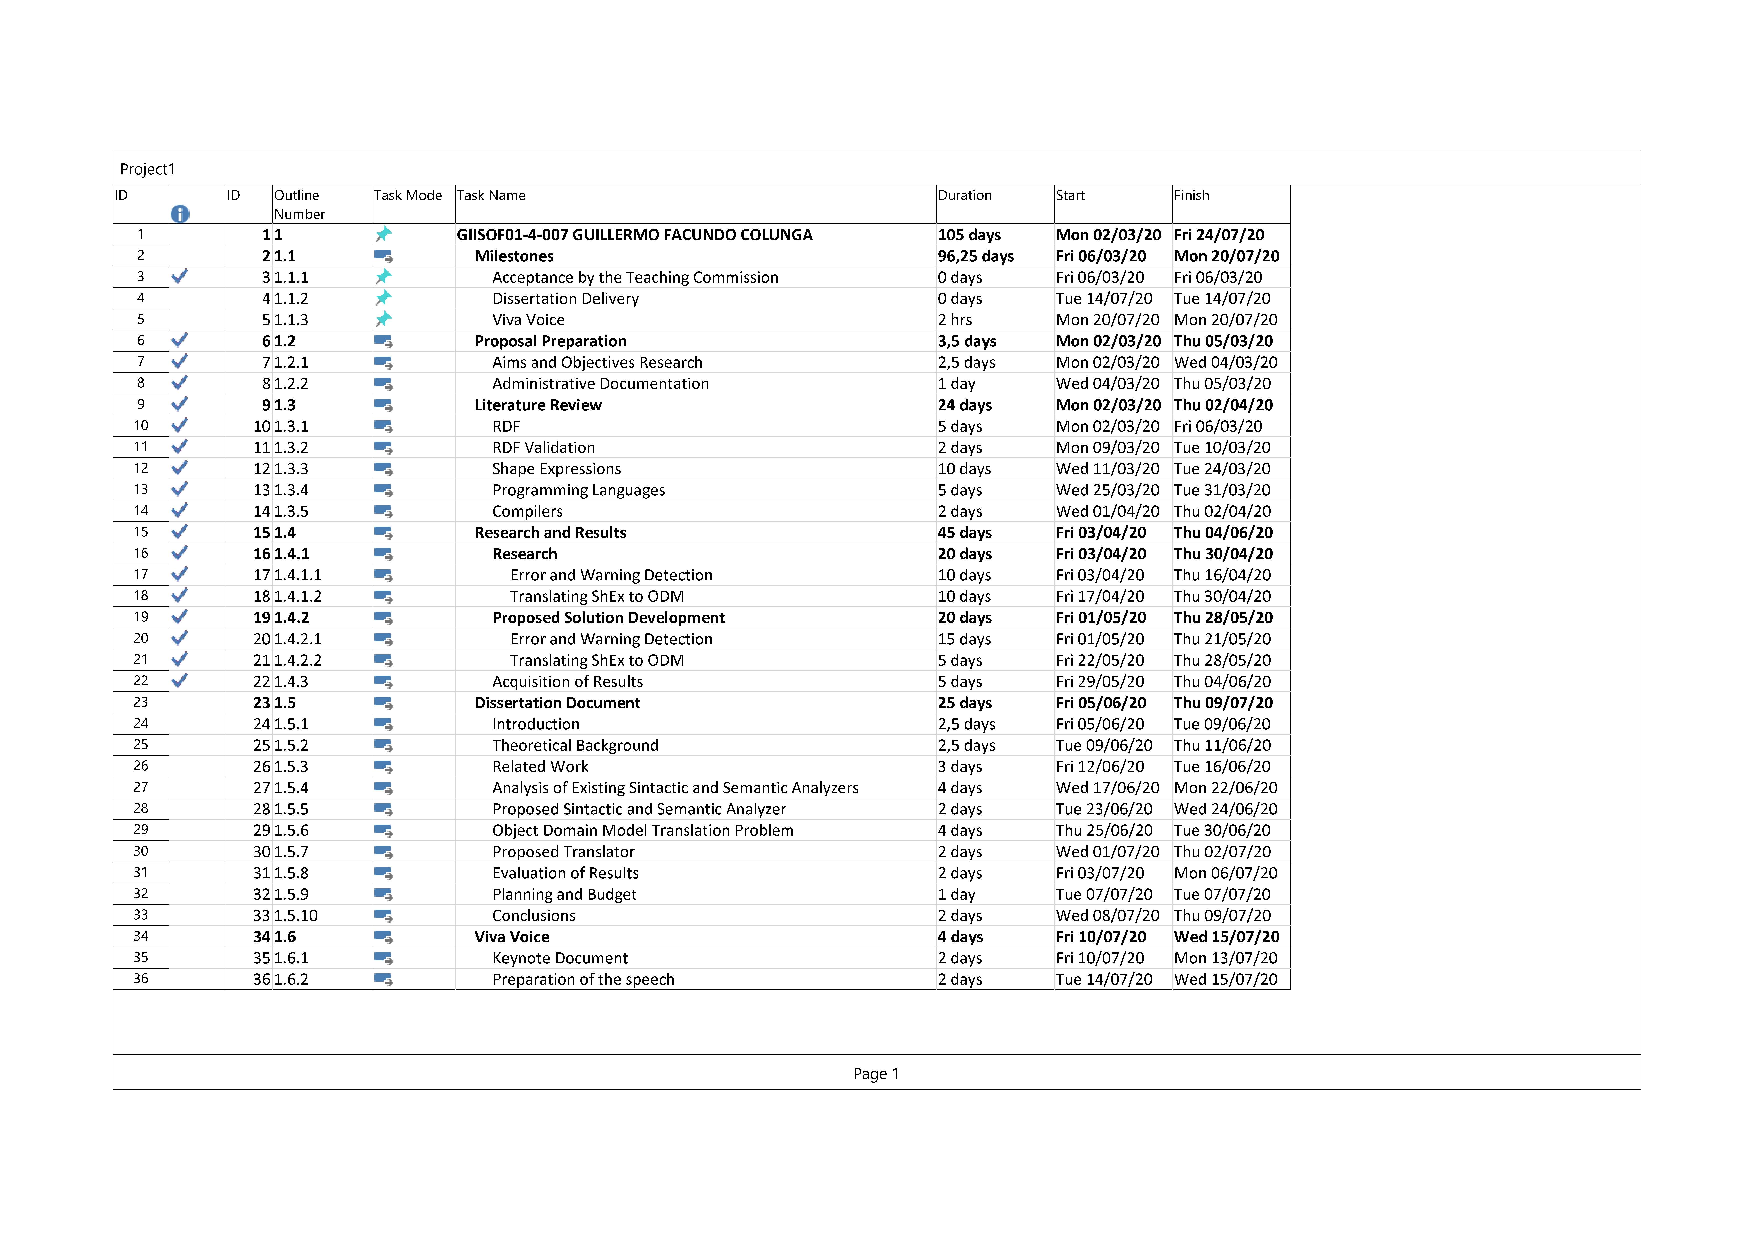
\includegraphics[width=\textwidth]{images/planificacion.pdf}
    \centering
	\caption[Tasks planning of the project]{Tasks planning of the project.}
    \label{fig:planning-sheet}
\end{figure}

\section{Budget}